%%%%% The Solution %%%%%

\chapter{Proposed Solution: A New Teaching Environment for Programming} \label{ch_pa}

In order to let students have a \emph{Sichtenwechsel} with relation to programming, \ie have them experience several different abstraction levels involved between a program's source code and its execution, a new teaching environment dubbed ``Processing Abstractions'' is proposed:

Within \ac{GT}, we've implemented support for the Processing programming language and molded views for every implementation step along the way. This allows for creating interactive notebook pages containing source code and a variety of these views, showing \eg the \ac{AST} and resulting bytecode for the \ac{GT} \ac{VM} side by side.

In this chapter, we document the architecture of this environment and the reasons for the approaches chosen. If you want to inspect the environment yourself, see appendix \ref{app_setup} for how to install all referenced code.\footnote{Remove the line \ct{GtExplorationHomeSection studentMode: true.} in order to also see our implementation notes.}



\section{Overview of ``Processing Abstractions''}

``Processing Abstractions'' consists of a transpiler for translating Processing source code into executable objects, a runtime environment, a large collections of views into various aspects of the program, and teaching materials using them.\footnote{The teaching materials currently provided are in the language used for teaching at the location of writing: German.} Tools and views as well as materials are all implemented within \acf{GT}, the former in Smalltalk code and the latter as ``Lepiter'' notebook pages.

\begin{cfigure}[fig_screenshot_vm_execution]{Excerpt from an interactive notebook page on program execution in a \ac{VM}.}
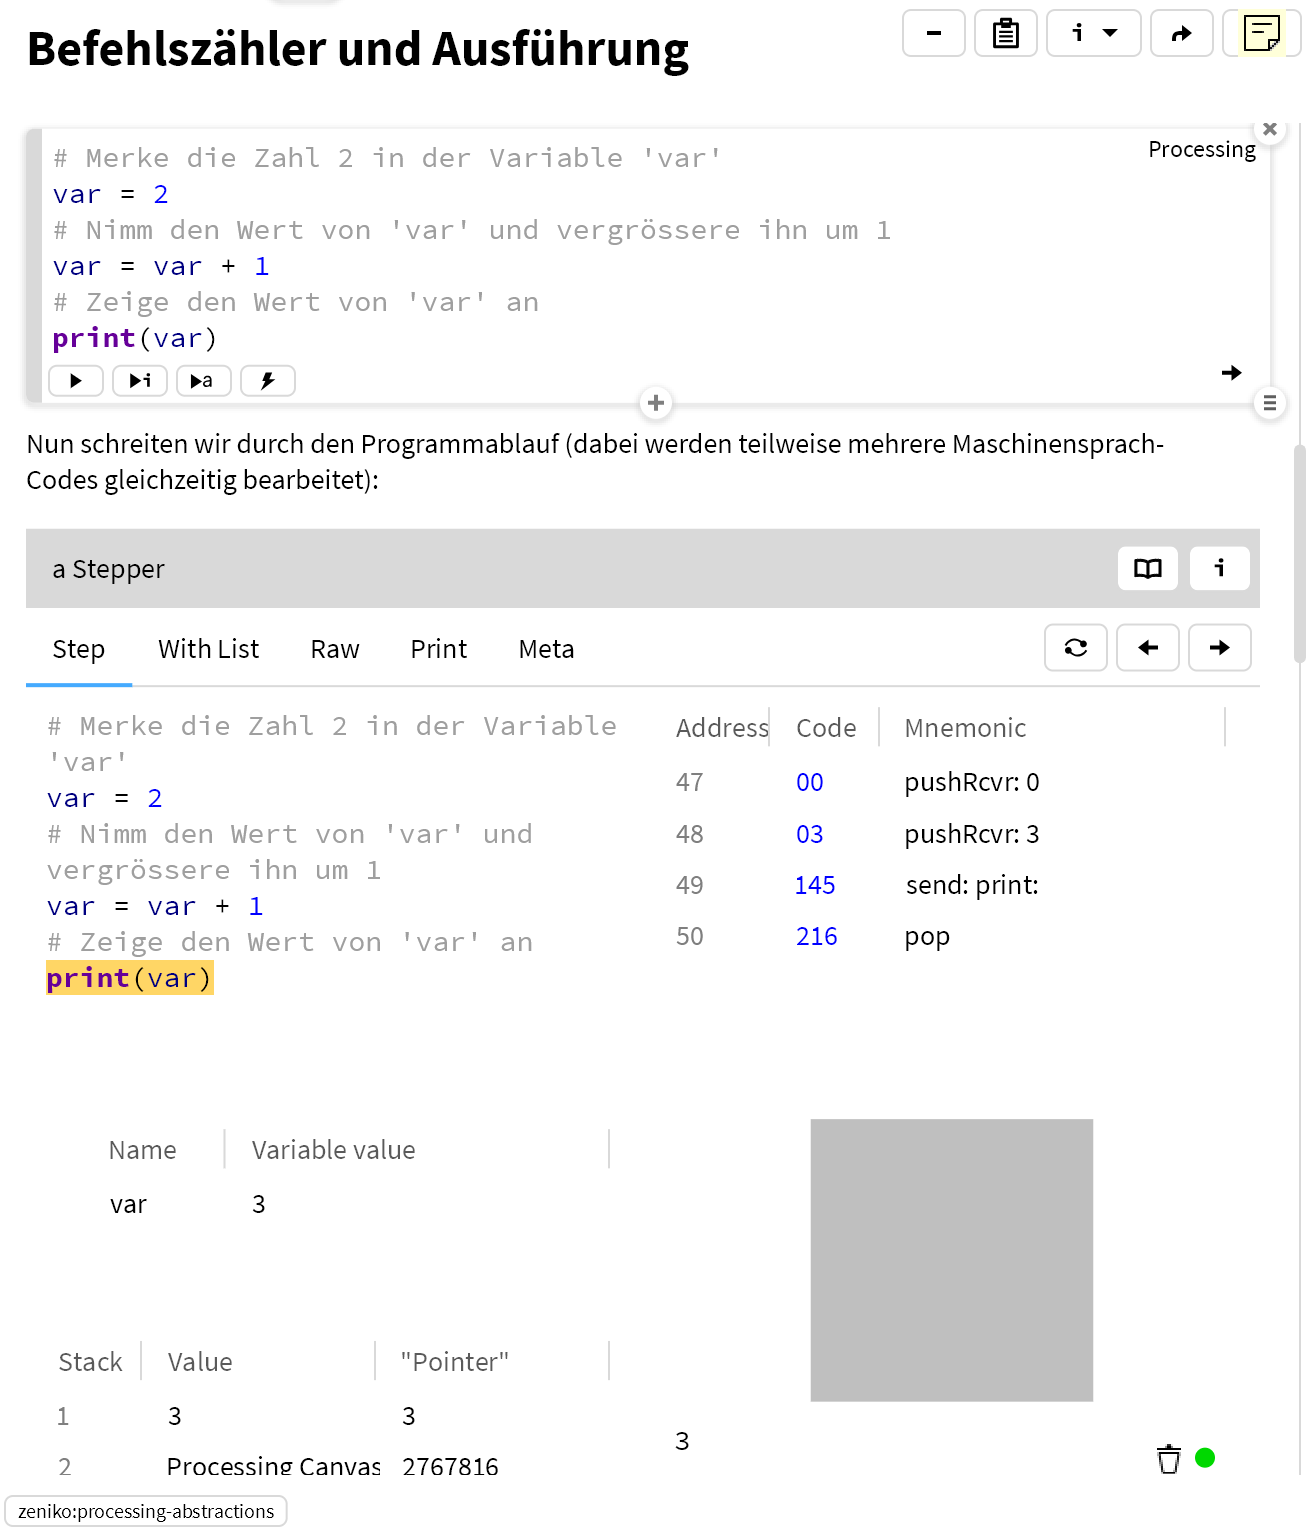
\includegraphics[width=.7\textwidth]{screenshot_vm_execution}
\end{cfigure}

Figure \ref{fig_screenshot_vm_execution} shows an excerpt from materials for students: The program visible at the top resides in a Processing-specific ``snippet'' with commands for running and inspecting the program independently of the page it resides on at the bottom; below a combined view for one execution step is shown with (clockwise) the step in question highlighted in source code; the corresponding bytecode visible; the program's output up to and including the current step; the contents of the execution stack of the Smalltalk \ac{VM}; and a list of all variable states.

Many such views are updated live whenever the source code is modified, without any other action required by students.\footnote{The one exception is the combined run-step view, which for longer running programs would be too resource intensive to regenerate on the fly. Refreshing it manually is still possible.} The five views shown in figure \ref{fig_screenshot_vm_execution} can also be used on their own or in other arrangements (\eg only source and a full bytecode view where interacting with one automatically highlights the corresponding items in the other).

As will be shown below, dozens of premade views are available. Any of them can be embedded in a notebook page by adding an ``Element'' snippet with the one line of Smalltalk code shown in figure \ref{fig_embedding_view}. As an example, this code connects the first Processing snippet on the current page with a live \ct{gtTreePlusSourceFor:} view.

\begin{cfigure}[fig_embedding_view]{Smalltalk code for embedding a view in a notebook page}
\begin{code}
(ProcessingSource fromPage: thisSnippet page at: 1) renderLiveView: #gtTreePlusSourceFor:
\end{code}
\end{cfigure}

From these views, interactive teaching materials related to programming, compilers and code execution in a (virtual) machine can be composed, allowing students to combine their preexisting knowledge from programming with concepts of different abstraction levels.



\section{Exploring Abstraction Levels}

Any of the views into a program require its source written in Processing with Python syntax\footnote{Restricted to the implemented API as documented in appendix \ref{app_api}.} available either as a single file or as snippet in a \ac{GT} notebook. We recommend the latter, as views are then generally live and effects of changing the source code can be more easily explored by students. An overview of available views is listed in figure \ref{fig_views_diagram}.

\begin{cfigure}[fig_views_diagram]{An overview of all the views and the order students will step through them}
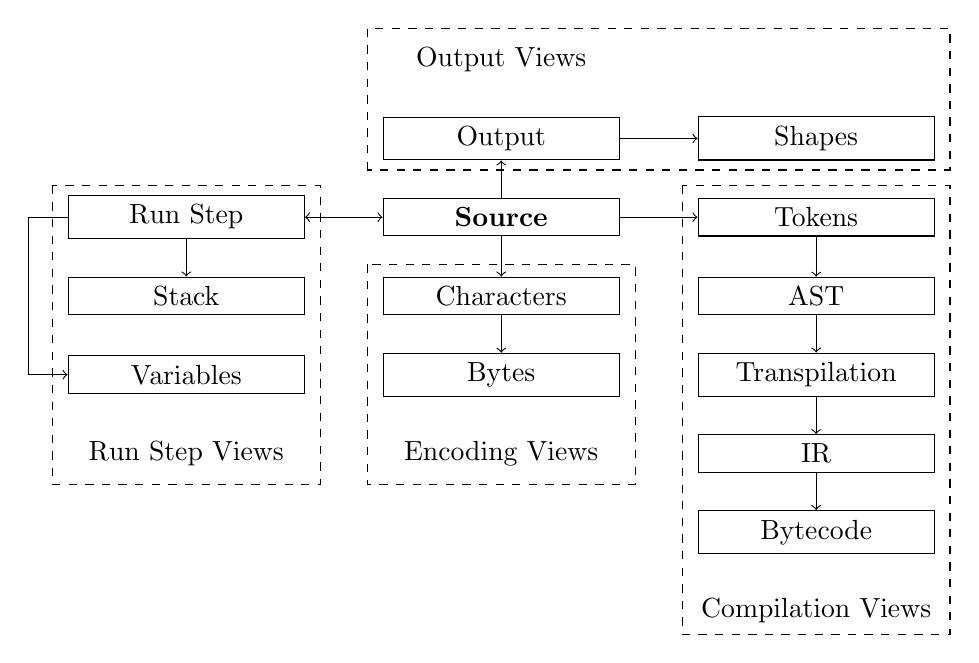
\begin{tikzpicture}

\node [draw, rectangle, minimum width=3cm] (source) at (0, 0) {\textbf{Source}};
\node [draw, rectangle, minimum width=3cm] (output) at (0, 1) {Output};
\node [draw, rectangle, minimum width=3cm] (tokens) at (4, 0) {Tokens};
\node [draw, rectangle, minimum width=3cm] (ast) at (4, -1) {\ac{AST}};
\node [draw, rectangle, minimum width=3cm] (transpilation) at (4, -2) {Transpilation};
\node [draw, rectangle, minimum width=3cm] (ir) at (4, -3) {\ac{IR}};
\node [draw, rectangle, minimum width=3cm] (bytecode) at (4, -4) {Bytecode};

\node [draw, rectangle, minimum width=3cm] (runstep) at (-4, 0) {Run Step};
\node [draw, rectangle, minimum width=3cm] (stack) at (-4, -1) {Stack};
\node [draw, rectangle, minimum width=3cm] (variables) at (-4, -2) {Variables};

\node [draw, rectangle, minimum width=3cm] (characters) at (0, -1) {Characters};
\node [draw, rectangle, minimum width=3cm] (bytes) at (0, -2) {Bytes};

\node [draw, rectangle, minimum width=3cm] (shapes) at (4, 1) {Shapes};

\draw [->] (source) -- (output);
\draw [->] (output) -- (shapes);
\draw [->] (source) -- (tokens);
\draw [->] (tokens) -- (ast);
\draw [->] (ast) -- (transpilation);
\draw [->] (transpilation) -- (ir);
\draw [->] (ir) -- (bytecode);
\draw [<->] (runstep) -- (source);
\draw [->] (runstep) -- (stack);
\draw [->] (runstep.west) -- +(-0.5, 0) |- (variables);
\draw [->] (source) -- (characters);
\draw [->] (characters) -- (bytes);

\draw [dashed] (-1.7, 0.6) rectangle (5.7, 2.4);
\node at (0, 2) {Output Views};
\draw [dashed] (2.3, 0.4) rectangle (5.7, -5.3);
\node at (4, -5) {Compilation Views};
\draw [dashed] (-1.7, -0.6) rectangle (1.7, -3.4);
\node at (0, -3) {Encoding Views};
\draw [dashed] (-5.7, 0.4) rectangle (-2.3, -3.4);
\node at (-4, -3) {Run Step Views};

\end{tikzpicture}

\end{cfigure}

Screenshots of all views can be found in appendix \ref{app_implementation}. Note that most views show a molded collection of objects that can be inspected individually by double-clicking the corresponding item.


\subsection{Source Snippet}

The ``Processing/Python'' snippet used in \ac{GT}'s notebook pages is the only place where Processing source code can be modified. It also provides several ways to run the program:

\begin{itemize}
\item {\small\faPlay} (or its shortcut \ct{Ctrl+R} for ``Run'') runs the program and either display its ``Output'' view or an inline error message.
\item {\small\faPlay}\texttt{i} (or its shortcut \ct{Ctrl+G} for ``debuG'') runs the program, recording all individual steps at the level of Python (sub)expressions -- allowing programmers to step through the program's runtime views and inspecting among other aspects the values of variables and the current state of the output.
\item {\small\faPlay}\texttt{a} (or its shortcut \ct{Ctrl+D} for ``Details'') shows the ``Abstractions'' view, \ie the program's main decomposition states: source code, \ac{AST}, bytecode, and output.
\item \lightning\ (or its shortcut \ct{Ctrl+Shift+D}) opens \ac{GT}'s Smalltalk debugger at the \ct{gtRun} entry point of the transpiled code for live debugging for either advanced students or for looking under the hood of the \ac{API} calls.
\end{itemize}

With just one source snippet, students can write and inspect programs with the opened views updating live as the program changes. This should give about the same experience as the Processing IDE with the main distinction that it is a live environment.

In contrast to the snippet, views are static in the sense that the source code can't be modified there.


\subsection{Output View}

The only views students should already know are the traditional ``Source'' and ``Output'' views, which show the source code and the result of running the program respectively. Programs containing an animation loop will show the animation and allow user interaction in any output view.\footnote{Interactions are currently limited to mouse movements and clicks.}

The ``Source'' view is meant to be linked to any other view, allowing for interacting between them by selecting source expressions and having the corresponding item(s) in the other view(s) also selected.

The ``Output'' view can be used at any state to quickly verify visually that a program behaves as expected, be it during an introduction to programming or when exploring part of a program's execution or decomposition.\footnote{All of these views are directly available for a Processing program when running it using {\small\faPlay}\texttt{a} or \ct{Ctrl+D} and then selecting the \texttt{i} selector at the top (see figure \ref{fig_gt_screenshot} on page \pageref{fig_gt_screenshot}).}


\subsection{Compilation Views}

One way to show students what happens to a program before it can be executed on a (virtual) machine is to take them through the involved steps:

\begin{itemize}
\item The ``Tokens'' view (see figure \ref{fig_views_parser}) shows each of the tokens the lexer has encountered, including additionally required information such as a line number and line indentation.\footnote{Indentation is relevant, as Python and as a consequence Processing with Python syntax is a language with significant whitespace, using common indentation for denotating code blocks.} This view can be used for students to see what a compiler is looking at in their program with whitespace and comments in particular missing.\footnote{As a limitation, tokens are currently extracted in reverse from the parser, which prevents inspecting tokens of syntactically invalid programs.}
\item The ``\ac{AST}'' view (see figure \ref{fig_views_parser}) shows the resulting parsing tree in a form that differentiates semantically relevant (sub)expressions from purely structural tokens. Combined with the ``Tokens'' view, this view can be used for hypothesizing and exploring how and what tokens are grouped together. In order to allow better interaction between ``Tokens'' and ``\ac{AST}'' views, the latter is a tree-list. A proper ``\ac{AST} Tree'' view is however also provided where the tree structure is more obviously visible, in particular also for larger programs.
\item The ``Transpilation'' view shows the result of translating the \ac{AST} to Smalltalk. Since the \ac{AST} needs to be barely modified for this translation step, Smalltalk code should be relatively easy to understand, at least when the original Processing source is displayed in parallel.

The ``Transpilation'' view also allows students to see what Processing does implicitly behind the scenes: setting and updating implicit variables, such as \ct{width}, \ct{mousePressed}, \etc, calling \ct{setup} once and \ct{draw} repeatedly, and running top-level code before entering the animation loop (see figure \ref{fig_views_gtRun}). Since \ac{GT}'s code component is used for displaying the transpiled code, this view has syntax highlighting and also allows users to explore the source code of called methods, letting students see that even presumably primitive commands can be implemented out of blocks (or in the case of \ct{whileTrue:} in figure \ref{fig_views_gtRun} on the basis of recursion).

In order to discuss programming language syntax, two additional views ``Prefix'' and ``Postfix'' show transpilations into a Lisp-like language using S-expressions and a Postscript-like language with reverse polish notation respectively. These may also serve as a basis for students' own parser projects, translating these pseudo languages back into Processing or Smalltalk.
\item The ``\acs{IR}'' view shows the \ac{IR} generated by the Smalltalk Opal compiler from the transpiled Smalltalk code. With function and variable names still showing and optimizations still missing, this allows students to make more sense of the eventual bytecode, in particular when both views are displayed side by side.
\item The ``Bytecode'' view finally show a list of the bytecodes that will be run by the Smalltalk \ac{VM}\footnote{Unless it is later translated to native code by the \ac{JIT}.} with instruction addresses\footnote{These are actually byte indices in the method's binary layout as used by the Smalltalk \ac{VM}.} and mnemonic added, so that jumps can be understood and the code can be more easily connected to either \ac{IR} or any other form of Assembly language. The bytecode of multiple methods is separated with the method name used as separator, as in the Smalltalk \ac{VM} addresses are counted starting at zero for every method.
\end{itemize}

All of these views can be linked together, so that selecting an item in one view will highlight the corresponding item(s) in the linked views. The default ``Abstractions'' view, available directly from every Processing snippet, \eg combines the source with ``\ac{AST}'', ``Bytecode'' and ``Output'' (visible on the right hand side in figure \ref{fig_gt_screenshot} on page \pageref{fig_gt_screenshot}, with a source expression and its corresponding items highlighted).

Being able to walk through all of these various compilation steps is something we haven't seen any \ac{IDE} offer. On the other hand, being able to connect this with an actually working program -- in the form of the ``Output'' view -- should offer students an explorable and interactive insight in a manageable package.

\begin{cfigure}[fig_views_parser]{Screenshot of a page of student content showing modifyable Processing source with live views for tokenization (left) and abstract syntax tree (right).}
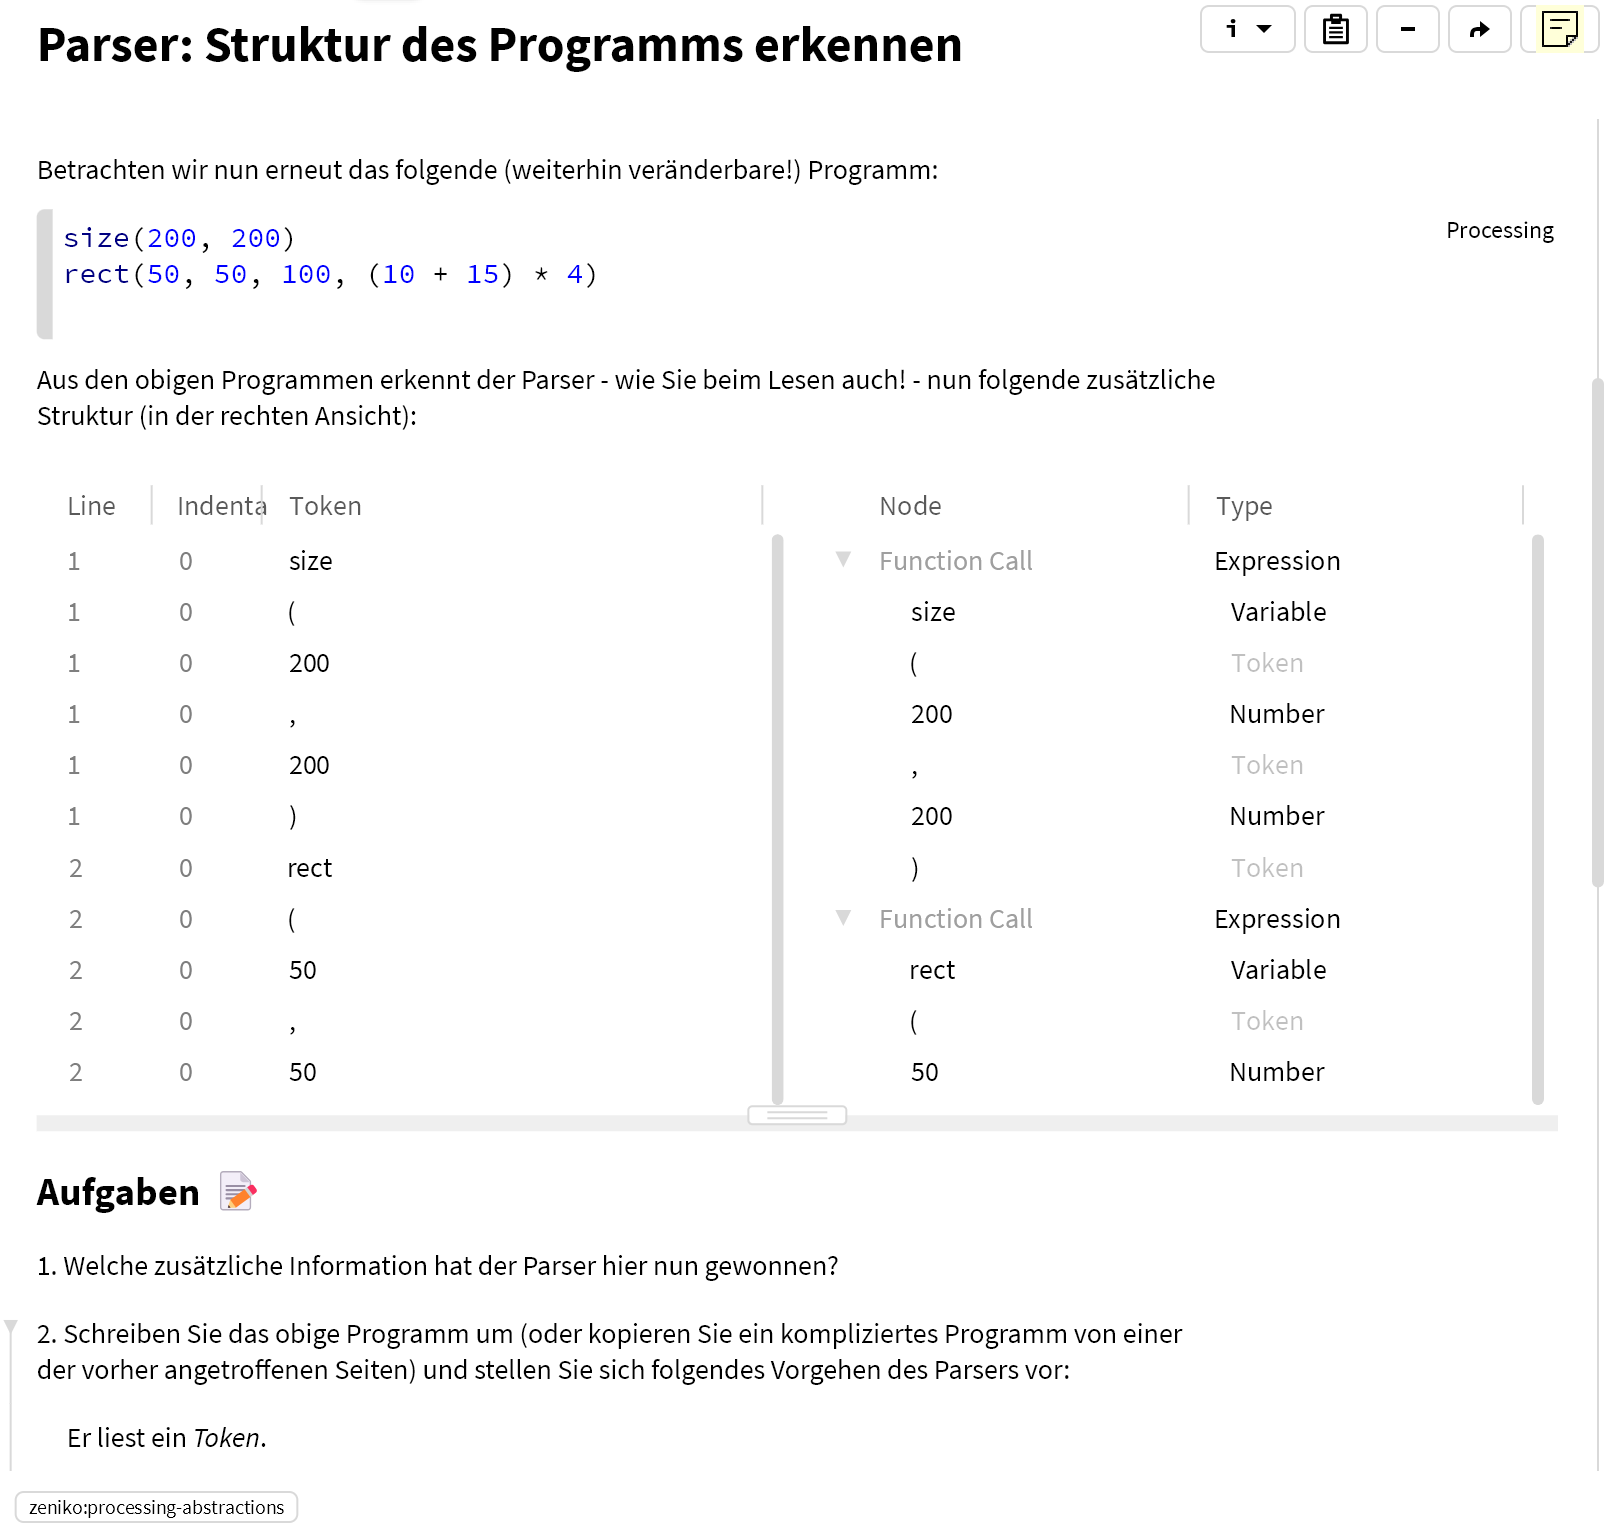
\includegraphics[width=.8\textwidth]{screenshot_parser}
\end{cfigure}

\begin{cfigure}[fig_views_gtRun]{Screenshot of a transpiled \ct{draw} method and the implicit animation loop}
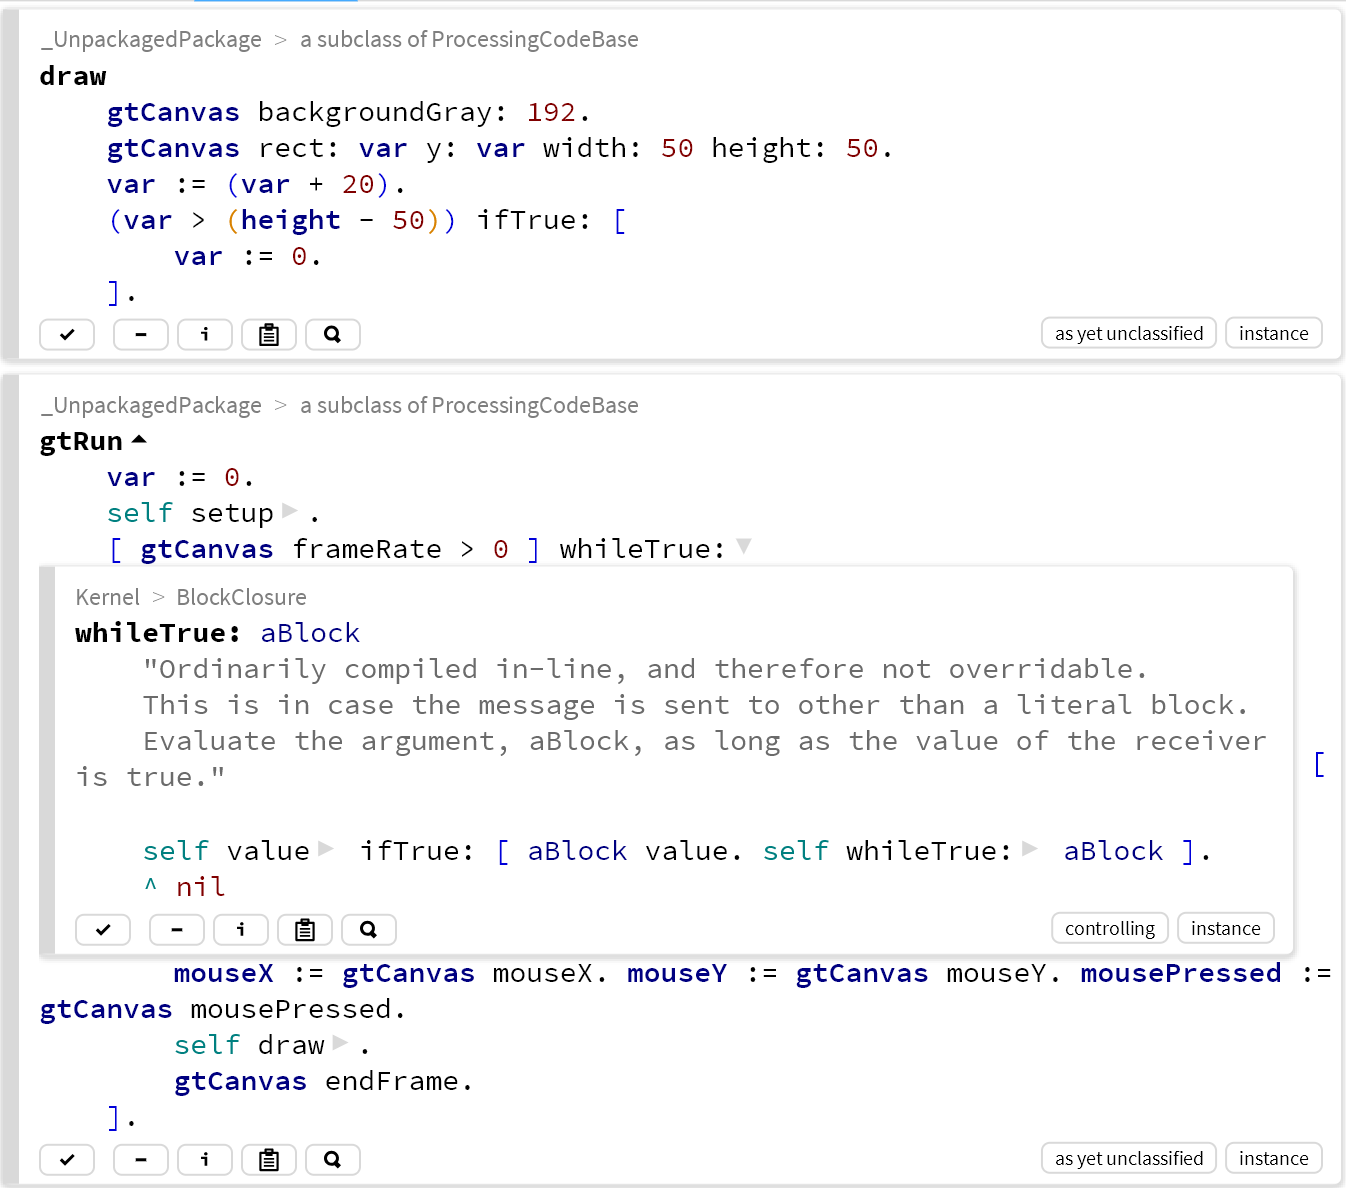
\includegraphics[width=.8\textwidth]{screenshot_gtRun}
\end{cfigure}


\subsection{Run Step Views}

Since in the background we have an actual translation of the Processing program to bytecode, which can be executed, we can also inspect the resulting execution. In contrast to the other views, this isn't live but a recording of a run, where we collect and show the following for every Processing (sub)expression being executed:

\begin{itemize}
\item The ``Source'' view shows the full source code with the (sub)expression in question being highlighted. This view is meant to be combined with any of the following views.
\item The ``Bytecode'' view shows only the bytecodes relevant for executing the current (sub)expression. This will show students not only into how many instructions a perceived single Processing instruction is compiled but also allow them to find that there's a calling convention that involves multiple instructions for every function call.\footnote{In the case of the Smalltalk \ac{VM}, this convention consists in pushing the ``receiver'', \ie the object being sent a message, to the stack and in the end cleaning the stack up if the call's result isn't needed.}
\item The ``Stack'' view shows the \ac{VM}'s value stack at the moment of a function call (\ie with the arguments already on the stack). For every stack argument a ``pointer'' value is also shown as a pseudo address, as effectively that's what the stack will contain. Since actual pointers aren't available from the Smalltalk \ac{VM}, these ``pointers'' are actually hashes (except for small integers, which students will have to discover can up to a point be used as themselves).
\item The ``Variables'' view shows the current values of all local and global variables (except for implicit variables for manageability reasons).
\item The ``Output'' view in this case shows the output state \emph{after} the step's execution, allowing students to better judge the effects of a function call.\footnote{Else they would have to switch between states to verify that the expected result has actually happened.}
\end{itemize}

Since a single program run usually takes many run steps, these views are meant to be displayed together in an interface allowing observers to step through the execution. For manageablility, when accessed directly from the Processing snippet, this combined view will not contain the ``Bytecode'' and ``Stack'' views. The full view will thus have to be shown explicitly to students once they have been introduced to the relevant concepts, whereas the reduced view can also be used for debugging the execution of a program during an introductionary programming course.


\subsection{Encoding Views}

For a different connection, source code can also be viewed as text that has to be stored somehow. To show this, there are two additional views to source code:

The ``Characters'' view lists the source code split into individual characters and shows characters with their Unicode value in decimal and hexadecimal. The hexadecimal notation is for a later comparison with either a binary file viewer\footnote{Such as \eg \url{https://hexed.it/}.} or with the ``Bytes'' view.

The ``Bytes'' view shows the UTF-8 encoding\footnote{UTF-8 is the default encoding of most modern software, in particular however it is the encoding chosen for both \ac{GT}'s notebook pages and for the Processing IDE.} of the source characters, as they are actually written to the disk. The bytes are again shown in their decimal and hexadecimal but also in binary notation. This is meant for students to combine programming also with text encoding lessons.


\subsection{Other Views}

Two further views are provided for delving deeper into the implementation of compiler and runtime:

The ``Slices'' view shows a list of all parsed Processing (sub)expressions with the corresponding transpiled expression. This list is used internally for matching Processing code to derivates of the transpiled Smalltalk.

The ``Shapes'' view shows a list of all shapes produced by a Processing program, demonstrating that in an object-oriented environment such as \ac{GT}, shapes aren't just collections of pixels but also objects with their properties, which can be handled independently.



\section{Implementation Details}

The environment consists of a Processing compiler and a runtime environment both implemented in Smalltalk inside \ac{GT}. Views were primarily implemented as close to the required data as possible but are all mirrored inside the main class \ct{ProcessingProgram} with a subset of these being shown for \ct{ProcessingSource}, which serves as entry class (see figure \ref{fig_uml_processing}).

%%%%% The Solution (UML Diagram) %%%%%

\newgeometry{bottom=1cm}

\begin{landscape}

\begin{cfigure}[fig_uml_processing]{Diagram of most classes involved in running Processing code within \ac{GT}}

\begin{tikzpicture}

\begin{package}{Processing}

\begin{class}[text width=6cm]{ProcessingSource}{0, 0}
\operation{fromFile:}
\operation{fromPage:at:}
\operation{fromSnippet:}
\end{class}

\begin{class}[text width=6cm]{ProcessingProgram}{0, 2.5}
\operation{ast}
\operation{compilation}
\operation{run}
\end{class}

\begin{class}[text width=6cm]{ProcessingParser}{-8, 0}
\operation{parse:}
\end{class}

\begin{class}[text width=6cm]{ProcessingTranspiler}{-8, 2.5}
\operation{transpile:}
\end{class}

\begin{class}[text width=6cm]{ProcessingTranspilationSlice}{-8, 7.5}
\operation{link:method:from:to:}
\end{class}

\begin{interface}[text width=6cm]{ProcessingCodeBase}{0, 5}
\operation{gtRun}
\end{interface}

\begin{class}[text width=6cm]{ProcessingRunner}{8, 5}
\operation{run:}
\operation{runSteps:}
\end{class}

\begin{class}[text width=6cm]{ProcessingCanvas}{0, 7.5}
\operation{asElement}
\operation{presenter}
\end{class}

\begin{class}[text width=6cm]{ProcessingCanvasPresenter}{8, 7.5}
\implement{ProcessingCanvas}
\end{class}

\begin{class}[text width=6cm]{ProcessingCanvasElement}{8, 9}
\end{class}

\begin{class}[text width=6cm]{ProcessingAstCleaner}{-8, 5}
\operation{clean:}
\end{class}

\begin{interface}[text width=6cm]{ProcessingCanvasShape}{0, 9}
\end{interface}

\begin{class}[text width=6cm]{ProcessingRunStep}{8, 2.5}
\end{class}

\draw[umlcd style dashed line, ->] (ProcessingSource) -- node[black]{$<<$accesses$>>$} (ProcessingProgram);
\draw[umlcd style dashed line, <->] (ProcessingProgram) -- node[black, sloped]{$<<$source $\rightarrow$ \ac{AST}$>>$} (ProcessingParser);
\draw[umlcd style dashed line, ->] (ProcessingProgram) -- node[black]{$<<$uses$>>$} (ProcessingTranspiler);
\draw[umlcd style dashed line, ->] (ProcessingTranspiler) -- node[black, sloped]{$<<$creates$>>$} (ProcessingCodeBase);
\draw[umlcd style dashed line, <->] (ProcessingTranspiler) -- node[black]{$<<$uses$>>$} (ProcessingAstCleaner);
\draw[umlcd style dashed line, ->] (ProcessingTranspiler.west) -- +(-1, 0) |- node[black, pos=0.25, sloped]{$<<$creates$>>$} (ProcessingTranspilationSlice);
\draw[umlcd style dashed line, ->] (ProcessingProgram) -- node[black]{$<<$accesses$>>$} (ProcessingCodeBase);
\draw[umlcd style dashed line, ->] (ProcessingProgram) -- node[black, sloped]{$<<$uses$>>$} (ProcessingRunner);
\draw[umlcd style dashed line, ->] (ProcessingRunner) -- node[black]{$<<$runs$>>$} (ProcessingCodeBase);
\draw[umlcd style dashed line, ->] (ProcessingRunner) -- node[black]{$<<$creates$>>$} (ProcessingRunStep);
\draw[umlcd style dashed line, ->] (ProcessingCodeBase) -- node[black]{$<<$owns$>>$} (ProcessingCanvas);
\draw[umlcd style dashed line, ->] (ProcessingRunner) -- node[black, sloped]{$<<$creates$>>$} (ProcessingCanvas);
\draw[umlcd style dashed line, ->] (ProcessingCanvas) -- node[black]{$<<$controls$>>$} (ProcessingCanvasPresenter);
\draw[umlcd style dashed line, ->] (ProcessingCanvasPresenter) -- node[black]{$<<$interacts$>>$} (ProcessingCanvasElement);
\draw[umlcd style dashed line, ->] (ProcessingCanvas) -- node[black]{$<<$creates$>>$} (ProcessingCanvasShape);
\draw[umlcd style dashed line, ->] (ProcessingCanvasShape) -- node[black]{$<<$renders$>>$} (ProcessingCanvasElement);

\end{package}

\end{tikzpicture}

\end{cfigure}

\end{landscape}

\restoregeometry


The implemented code can be found within \ac{GT}'s Coder (package manager) or by name through the Spotter (search engine (\faSearch)).\footnote{After it has been imported as described in appendix \ref{app_setup}. Note that a stable snapshot of the code discussed here is available at \url{https://github.com/zeniko/gt-exploration/tree/thesis}.}


\subsection{Processing Compiler}

Compiling a Processing program happens automatically when loading a source as a \ct{ProcessingSource} from snippet, file or string and then sending the source a \ct{program} message. Alternatively, the following steps can also be performed manually:

The Processing compiler mainly uses \ac{GT}'s builtin \ct{PythonParser} class for parsing the code, which is based upon the SmaCC parser generator.\footnote{\emph{Cf.} \archivedurl{https://refactory.com/smacc/}.} \ct{ProcessingParser} is a transparent subclass, allowing us to intermittently fix issues encountered in the Python parser.\footnote{It should be noted: All reported parser issues have been fixed within a day.}

The resulting \ac{AST} is then passed to \ct{ProcessingTranspiler}, which first rewrites the constructs that Smalltalk doesn't support: in-place arithemtics (\eg \ct{a += 2} is expanded to \ct{a = a + 2}) and unreachable statements after a \ct{return}, which have to be removed. Additionally, logical \ct{and} and \ct{or} operations are converted from being left associated (as per Python's precedence table) to being right associated, which \ac{GT} suggests for more efficiently handle early exits.\footnote{The Smalltalk compiler doesn't seem to optimize this case. We have not been able to verify whether the optimizing JIT does.} This rewritten \ac{AST} is only used internally and not visible to users.

Transpiling happens by a tree visitor, translating the individual \ac{AST} nodes to corresponding Smalltalk with no optimizations. For each node, a \ct{ProcessingTranspilationSlice} is recorded that contains a reference to the \ac{AST} node and the text span in the transpiled code.

Finally, an anonymous subclass of \ct{ProcessingCodeBase} is created and all Processing functions are then compiled from the transpiled code by the \ct{OpalCompiler} to executable methods. Global Processing code is compiled into the \ct{gtRun} entry point method and, if \ct{setup} and/or \ct{draw} functions are defined in Processing code, the implicit animation loop is also added.\footnote{In order to prevent overriding of \ct{gtRun} and the different view messages, Processing names starting with \ct{gt} are renamed to starting with \ct{gt_} during transpilation.} Processing \ac{API} calls -- if not overwritten by user code -- are translated through messages of the form \ct{ProcessingTranspiler>>>emit_...:}, which the transpiler detects through reflection.

The compiled object can be used as any object. In particular, \ac{GT}'s reflective capabilities can be used, \eg for extracting bytecodes of a method through \ct{CompiledCode>>>symbolicBytecodes}. \ct{ProcessingCodeBase} thus implements all views related to the Smalltalk \ac{VM}.

\ct{ProcessingProgram} mirrors those views and only implements views related to Processing code. In order not to overwhelm students with too many views, \ct{gtDefaultInspectorTool} has been implemented on \ct{ProcessingProgram} for hiding all but the main ``Abstractions'' combination view behind the same symbols as used by the snippet.

During compilation, most common exceptions are \ct{SmaCCParserError} during parsing, \ct{ProcessingCompileTimeException} during transpilation and \ct{ProcessingRunTimeException} during execution.


\subsection{Processing Runtime}

The Processing runtime consists of \ct{ProcessingRunner} and \ct{ProcessingCanvas}:

The runner moves code execution to a worker thread, leaving the UI thread available for output and interaction, and performs a simple heuristic for detecting accidental endless loops by simply terminating any program with too long a runtime. This is necessary in a live programming environment, as during composition students will almost inevitably write endless loops. The runner can also be used for extracting runtime steps. In order to achieve this, \ac{GT}'s debugging facilities for stepping through code are called and a debugging session is executed step-by-step in the background. For both users, the runner is automatically called by \ct{ProcessingProgram}.

The canvas provides the implementation of most of the Processing \ac{API}: Every compiled Processing program is assigned a canvas by the runner and all Processing \ac{API} calls are forwarded to the canvas for rendering. The canvas is implemented using the model-presenter-view pattern, allowing for multiple views for a single canvas. Shapes are thus also only abstractly created by the canvas, being instantiated by the presenter in every single view instance.


\subsection{Views}

All views in \ac{GT} are by convention provided by methods with names of the form \ct{gt...For:} and are categorized as ``views'' in the class browser.\footnote{Actual requirement is only the \ct{<gtView>} pragma annotation and the method signature (\ct{GtPhlowView} $\rightarrow$ \ct{GtPhlowView}).}

With any view visible in \ac{GT}, \ct{Alt}+clicking on a view's name shows its source method(s), revealing the view's method name and implementation. The method name will be required for embedding a view in a notebook page as described in figure \ref{fig_embedding_view} above.

For comparing the same views of different programs, the \ct{ViewComparison} helper class is provided, which can be used in ``Element'' snippets as follows:

\begin{code}
ViewComparison newFor: {
	(ProcessingSource fromPage: thisSnippet page at: 1) program -> #gtSourceCharsFor:.
	(ProcessingSource fromPage: thisSnippet page at: 2) program -> #gtSourceCharsFor:.
}
\end{code}


\subsection{Snippet}

The ``Processing/Python'' snippet is implemented through \ct{LeProcessingSnippet} and associated classes.\footnote{\emph{Cf.} figure \ref{fig_uml_snippet} on page \pageref{fig_uml_snippet}.} This is mostly based on the provided \ct{LePythonSnippet}, replacing the use of the Python language bridge with calls to our own Processing compiler and runtime.

The snippet can either create \ct{ProcessingSource} instances by itself, showing either the ``Output'', ``Runsteps'' or ``Abstractions'' views; or its code can be programmatically loaded in a notebook ``Element'' snippet as shown in figure \ref{fig_embedding_view}.\footnote{The \ct{at: 1} part of the message may also be omitted, if there's only one snippet on a notebook page. Inspect the ``views'' category of \ct{ProcessingProgram} in the coder or consult appendix \ref{app_implementation} for a full list of availble view names.}



\subsection{Other approaches considered}

Since Processing implemented on top of Python is a strongly but dynamically typed language, it maps well onto Smalltalk. Still, initially three other approaches were considered:

Processing could be run either in the original \ac{JVM} and then accessed through Python or directly run using one of several Python libraries \cite{Tab22}. In all cases, its objects would be accessed through \ct{PythonBridge}. Unfortunately at the time of writing, support for PythonBridge under Windows was difficult to achieve in a portable manner (\ie without requiring students to install multiple different packages, which increases the risk of accidental breaking and thus potential support issues). Additionally, \ct{PythonBridge} only gives access to dictionaries of serialized Python object properties, which would have required a potentially slow level of indirection involved when running and inspecting animations.

Alternatively, Processing could have been implemented through an interpreter in \ac{GT}.\footnote{Remnants of which are available as \ct{ProcessingInterpreter}.} This would have required to write a separate compiler for creating bytecode just for demonstration purposes.

As a third option, a compiler from Processing to Smalltalk bytecode could have been written.\footnote{A compiler for a tiny subset of Processing is included as \ct{ProcessingCompiler}.} While this would have allowed for closer control over optimizations, it would effectively have become a reimplementation of most of \ct{OpalCompiler}.



\section{Potential Drawbacks}

Since \ac{GT} is based on Smalltalk, an initial effort is required to learn language and environment before their benefits can be used. This is helped by Smalltalk's regular syntax and \ac{GT}'s reflective capabilities.\footnote{For Smalltalk and \ac{GT}'s ancestor Pharo, there are sufficient resources available online, for \ac{GT} itself, there's the ``Glamorous Toolkit Book'' \cite{Gir23} and a Discord server.}

Modrow and Strecker \cite{Mod16} prefer a block based language in order to prevent students from getting lost in syntax errors. This issue has at least been remedied partially by having a live environment. Error messages are however not in optimal shape yet, sometimes rather hinting at an issue than explaining it as Bouvier \etal \cite{Bou24} call for.

Chiodini \etal \cite{Chi23} also propose starting with visual programming but have different requirements: In order to keep an introductionary language manageable, they ask among other things for a limited \ac{API} that should be expandable by students (see also \ref{ssc_manageability}). And the full Processing \ac{API} can indeed be quite overwhelming, so only a subset must be introduced at the start. Indeed also for this reason only a subset has been implemented in \ac{GT} (see appendix \ref{app_api}).

Another requirement by Chiodini \etal is for problems to be transparently decomposed and solutions recomposed. This is indeed an issue with Processing: Moving a composed shape to a different location requires adjusting the coordinates of all basic shapes involved, therefore variables and even functions have to be introduced sooner rather than later to allow the examples shown \cite{Chi23} to work. Similar to how they introduce a library to achieve their desired \ac{API}, the same functionality could be implemented on top of Processing at a later stage if desired.\footnote{In the provided teaching materials, an example of how to implement a simpler Turtle based \ac{API} is provided (see ``Schildkr�ten und Rekursion''), however even Turtles have state, which makes composition non-trivial.}

The main reason for not introducing a new \ac{API} as proposed by Chiodini \etal is the same as the reason for not introducing an entirely new programming language optimized for teaching (as done \eg by Black and Bruce \cite{Bla18}): This prevents benefiting from the large community and preexisting documentation and example code.

Using \ac{GT} for students also means introducing a new environment, which might introduce new pitfalls and adds additional cognitive tax on students.
